\setauthor{Moritz Eder}
\begin{spacing}{1}
    \chapter*{Abstract}
\end{spacing}
\begin{wrapfigure}{r}{0.3\textwidth}
    \begin{center}
      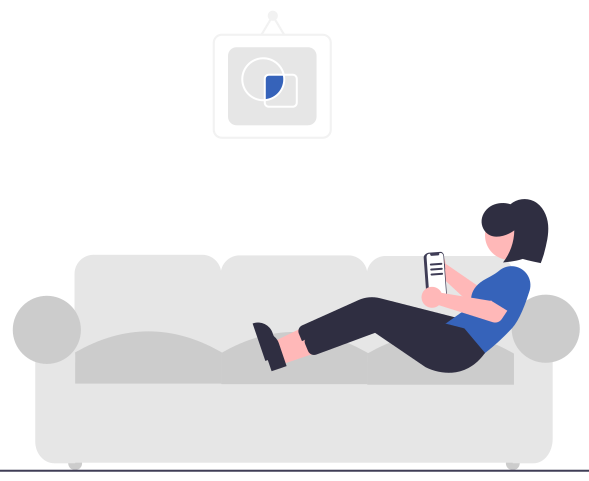
\includegraphics[width=0.3\textwidth]{pics/undraw_Relaxing_at_home_re_mror.png}
    \end{center}
\end{wrapfigure}
<Coming soon>
\newpage
\begin{spacing}{1}
    \chapter*{Zusammenfassung}
\end{spacing}
\begin{wrapfigure}{r}{0.3\textwidth}
    \begin{center}
      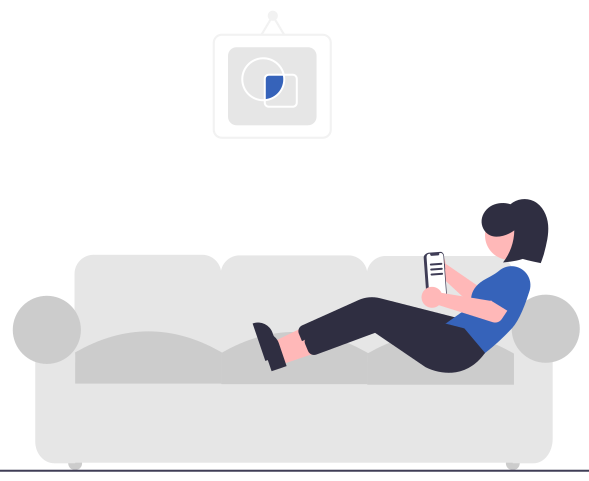
\includegraphics[width=0.3\textwidth]{pics/undraw_Relaxing_at_home_re_mror.png}
    \end{center}
\end{wrapfigure}
Relaxoon ist ein Wortspiel aus den englischen Wörtern 'relax' und 'soon'. 

Relaxoon bietet Entspannungsübungen in Form von Videos, Texten, Artikeln und noch mehr. 
Dabei ist ein sehr userfreundliches beziehungsweise simples User-Interface eins der größten Besonderheiten von Relaxoon.

